\documentclass[11pt]{article}
% Venue-neutral skeleton. Switch to the venue style file once the target is fixed.
\usepackage[margin=1in]{geometry}
\usepackage{amsmath,amssymb,amsthm}
\usepackage{graphicx,booktabs,xcolor}
\usepackage[round]{natbib}
\usepackage[hidelinks]{hyperref}

\newtheorem{proposition}{Proposition}
\newtheorem{lemma}{Lemma}
\newtheorem{theorem}{Theorem}
\newtheorem{corollary}{Corollary}
\theoremstyle{definition}
\newtheorem{definition}{Definition}
\theoremstyle{remark}
\newtheorem{remark}{Remark}

\newcommand{\hole}[1]{\textcolor{red}{[#1]}}
\DeclareMathOperator{\lse}{lse}
\DeclareMathOperator{\softmax}{softmax}
\newcommand{\R}{\mathbb{R}}

\title{Calibrated Steering Paths Reveal Complementary Failure Modes of Out-of-Distribution Detectors}
\author{\hole{Authors}}
\date{}

\begin{document}
\maketitle

\begin{abstract}
Out-of-distribution (OOD) detectors are usually compared with static metrics such as AUROC. These metrics
average over an unspecified mixture of distribution shifts and do not identify which shifts a detector misses.
We instead measure detectors along shared, declared paths in representation space. In-distribution features
are steered along a path, every detector is calibrated to the same in-distribution rejection rate, and we
record the distance at which each first rejects. A detector depends on its input only through the features,
so a path that it never rejects implies blindness to every input shift that realises that path. Decomposing
paths into radial and angular components, we show that for linear-head energy and Euclidean distance scores,
radial growth drives energy toward acceptance and distance scores toward rejection. Radial shrinkage drives
distance scores toward their value at the origin and energy toward a constant set by the classifier's biases
alone. We give exact conditions for each detector's decision at the origin, and show that calibrated energy
decisions depend on a component of the classifier that leaves every prediction unchanged. Across four text
and four vision encoders and three independent seeds, every stated origin condition matches the observed
decisions, and distance-based and logit-based detectors fail along different paths.
\end{abstract}

\section{Introduction}
% P1 Problem. \hole{}
% P2 Gap: static AUROC averages over an unknown mixture of shifts. \hole{}
% P3 Why representation space: Lemma~\ref{lem:reduction}; realisation is a tube condition
%    (Def.~\ref{def:realise}), not endpoint proximity.
% P4 Why shared, declared paths: paired comparison; polar basis (Table~\ref{tab:polar}).
% P5 Why calibrated comparison: Prop.~\ref{prop:invariance}; its limit is Prop.~\ref{prop:gauge}.
% P6 \hole{Instrument summary.}
% P7 Complementarity: Prop.~\ref{prop:radial}.
% P8 Contributions:
% (1) Instrument + validity: calibrated first rejection on shared paths;
%     invariance (Prop.~\ref{prop:invariance}), crossing stability
%     (Thm.~\hole{stability}), error decomposition (Prop.~\hole{anova});
%     reduction to input shifts (Lemma~\ref{lem:reduction}) and its
%     $\epsilon$-realisation corollary for Lipschitz scores.
% (2) Polar analysis of paths: radial vs angular components; complementarity
%     of distance- and logit-based detectors (Prop.~\ref{prop:radial}),
%     with exact origin conditions for kNN, Mahalanobis, energy and MSP.
% (3) Energy-specific structure: single flagged interval, cone condition for
%     eventual rejection (Thm.~\ref{thm:cone}), dependence on a
%     prediction-invariant component of the head (Prop.~\ref{prop:gauge}).
% (4) Evidence on four text and four vision encoders, including
%     norm-controlled paths and an ID-support analysis of angular paths.

\section{Method: calibrated first rejection along declared paths}\label{sec:method}

\subsection{Detectors and calibration}
A frozen encoder $f$ maps an input to a feature $z=f(x)\in\R^d$, written in polar form $z=\rho u$ with
$\rho=\|z\|$ and $\|u\|=1$. In-distribution (ID) training data are split into disjoint pools: a head pool
for training a linear classifier with logits $Wz+b$ (rows $w_c$; $a=Wz$ denotes the bias-free logits),
a reference pool $\mathcal{D}$ for fitting distance-based detectors, a direction pool $\mathcal{V}$ for
estimating steering directions, a calibration pool $\mathcal{C}$ and a probe pool $\mathcal{P}$ of ID
points to be steered. Test sets are used only for static evaluation.

We study four scores, all oriented so that larger means more anomalous.
\begin{itemize}
\item \emph{kNN}~\citep{sun2022knn}: the Euclidean distance to the $k$-th nearest point of $\mathcal{D}$,
on unnormalised features.
\item \emph{Mahalanobis}~\citep{lee2018mahalanobis}: $\min_c (z-\mu_c)^\top P(z-\mu_c)$, with class
means $\mu_c$ of $\mathcal{D}$ and $P$ the inverse of the pooled within-class Ledoit--Wolf
covariance~\citep{ledoit2004}, computed in double precision.\footnote{The single-precision implementation of
\citet{kirchheim2022pytorchood} inverts an unregularised scatter matrix. On our full-dimensional vision
features this matrix is so ill-conditioned that the calibrated thresholds are off by more than an order of
magnitude. We do not use it.}
\item \emph{Energy}~\citep{liu2020energy}: $E(z)=-\lse(Wz+b)$.
\item \emph{MSP}~\citep{hendrycks2017baseline}: $M(z)=-\max_c\softmax(Wz+b)_c$.
\end{itemize}
Every score $S$ is thresholded at the $\lceil(m+1)(1-\tau)\rceil$-th order statistic $t$ of its $m$
calibration scores, for a common target rate $\tau$. The decision is $\delta(z)=\mathbf{1}[S(z)>t]$. Under
exchangeability this bounds the marginal ID rejection rate by $\tau$, and it puts every detector on the same
operating point regardless of its scale (Proposition~\ref{prop:invariance}). All settings are listed in
Appendix~\ref{app:impl}.

\subsection{Declared path families}
A path $\gamma:[0,H]\to\R^d$ starts at a probe, $\gamma(0)=z$. We use four families
(Table~\ref{tab:polar}), each fixed before measurement and shared by all detectors:
\begin{itemize}
\item straight rays $\gamma(\alpha)=z+\alpha v$;
\item geodesics on the sphere of radius $\rho$, $\gamma(\alpha)=\rho\,(\cos(\alpha/\rho)\,u+\sin(\alpha/\rho)\,w)$,
with $w$ the normalised component of $v$ orthogonal to $u$ and $\alpha$ the arc length, so that
$\|\gamma(\alpha)\|=\rho$;
\item paths toward the origin, $\gamma(\alpha)=z-\alpha u$;
\item radial growth, $\gamma(\alpha)=z+\alpha u$.
\end{itemize}
For straight rays and geodesics, $v$ is either the top principal direction of a bootstrap resample of
$\mathcal{V}$ (``PC'') or an isotropic random unit vector (``random''), and both signs $\pm v$ are used.
Distances are measured in ID radii, $\bar r=\operatorname{median}_{z\in\mathcal{D}}\|z-\bar z_{\mathcal{D}}\|$,
which makes encoders comparable. The horizon $H$ is a fixed multiple of $\bar r$ chosen on ID data only.
Paths toward the origin stop just short of it, and geodesics stop short of the antipode.

\subsection{Measuring first rejection}
Each path is evaluated on a uniform grid of $\alpha\in[0,H]$. The first grid crossing of $t$ is refined by
bisection to give $\alpha^*=\inf\{\alpha:\delta(\gamma(\alpha))=1\}$. A path never rejected on $[0,H]$ is
right-censored at $H$, and a probe rejected at the start has $\alpha^*=0$. We report the rejection rate
$R(\alpha)$, the fraction of steered probes with $\delta(\gamma(\alpha))=1$. Unlike the cumulative
first-rejection rate, $R$ decreases when a detector re-accepts a path. To compare path families with
different reachable lengths, we report $R$ at the \emph{matched horizon} $\alpha_m$: the largest $\alpha$
reached by every path family, encoder and seed, using the last grid point not beyond it.

\subsection{Design and statistics}
For each encoder and seed we use a crossed design:
\begin{itemize}
\item several stratified bootstrap resamples of $\mathcal{D}$ (detectors refitted, thresholds recalibrated
on the fixed $\mathcal{C}$);
\item several bootstrap resamples of $\mathcal{V}$ (direction estimates);
\item a fixed set of probes and both direction signs.
\end{itemize}
Radial families depend on neither $v$ nor its sign and use one of each. Three independent seeds
re-partition the data, retrain the head and redraw all resamples and probes. We report means over encoders
and seeds with hierarchical bootstrap confidence intervals that resample encoders, then seeds within each
encoder.

Every detector sees the same probes and paths, so comparisons between detectors are paired. For each
(seed, encoder) cell we bootstrap probes to obtain a one-sided $p$-value for the stated direction. We then
report in how many cells the difference is significant at the conventional level, together with a
hierarchical interval for the mean difference.

\paragraph{Verification.} In every run we refit the detectors independently and recompute the score at
randomly chosen path points. The result must match the traced scores, and the score at $\alpha=0$ must
match the unsteered probe score.

\subsection{Validity of the measurement}
\begin{lemma}[Reduction]\label{lem:reduction}
If an input shift $x(\beta)$ satisfies $f(x(\beta))=\gamma(\tau(\beta))$, then
$\delta(f(x(\beta)))=\delta(\gamma(\tau(\beta)))$ for all $\beta$. Hence a feature path that is never rejected
on $[0,H]$ implies that every input shift realising it on $[0,H]$ is never rejected.
\end{lemma}

\begin{definition}[$\epsilon$-realisation]\label{def:realise}
An input shift $\epsilon$-realises $\gamma$ if there is a monotone $\tau$ with
$\sup_\beta\|f(x(\beta))-\gamma(\tau(\beta))\|\le\epsilon$.
\end{definition}

\begin{corollary}
If $S$ is $L$-Lipschitz, decisions along $x(\beta)$ and $\gamma(\tau(\beta))$ agree wherever
$|S(\gamma(\tau(\beta)))-t|>L\epsilon$. For kNN, $L=1$; for energy, $L=\max_c\|w_c\|$.
\end{corollary}

\begin{proposition}[Invariance]\label{prop:invariance}
For strictly increasing $g$, the calibrated decisions of $g\circ S$ and $S$ coincide, and so do their $\alpha^*$.
\end{proposition}

\begin{proposition}[Gauge]\label{prop:gauge}
Replacing every $w_c$ by $w_c+r$ leaves the softmax, the predictions and MSP unchanged, and changes energy
to $E_r(z)=E(z)-r^\top z$. Since $r^\top z$ depends on the input, calibrated energy decisions can differ
between two heads that make identical predictions. At the origin $E_r(0)=E(0)$, but the calibrated
threshold $t_r$ moves with $r$, so the origin decision $-\lse(b)>t_r$ is gauge-dependent (Fig.~\ref{fig:polar}c).
\end{proposition}

\section{Polar analysis of paths}
\begin{figure}[t]
\centering
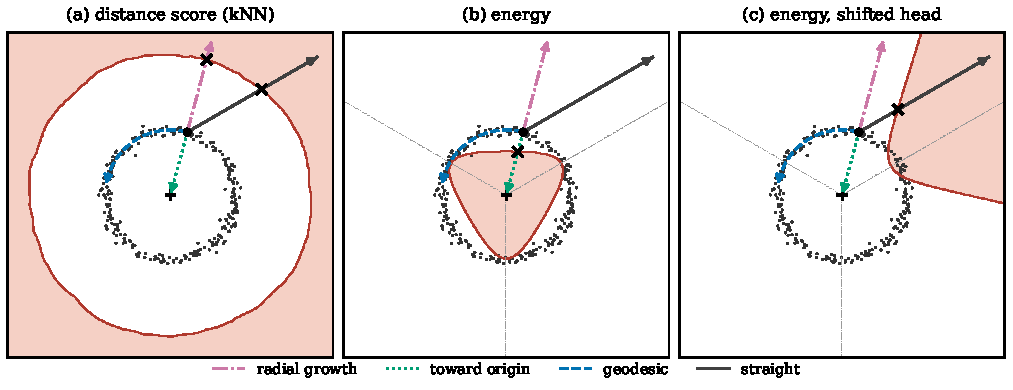
\includegraphics[width=\linewidth]{figures/fig_polar.pdf}
\caption{Schematic rejection regions (shaded) in two dimensions for ID features on a shell, with four
paths from one probe (dot); crosses mark first rejection. (a) A distance score rejects radial growth and
straight paths but accepts the origin (threshold set as in high dimension, $t>\rho$). (b) Linear-head energy
with rows summing to zero rejects only a bounded region around the origin. (c) The same head with every row
shifted by a common vector: predictions (dotted argmax boundaries) are unchanged, but the calibrated rejection
region moves (Prop.~\ref{prop:gauge}). The shifted head no longer rejects the path toward the origin, although
$E_r(0)=E(0)$, because the threshold is recalibrated.}
\label{fig:polar}
\end{figure}

\begin{table}[t]
\centering
\caption{Path families by their effect on the norm $\rho$ and the direction $u$ of $z=\rho u$.}
\label{tab:polar}
\begin{tabular}{lll}
\toprule
 & angular: no & angular: yes \\
\midrule
radial $+$ & radial growth $z+\alpha u$ & straight rays, $u^\top v\ge 0$ \\
radial $0$ & (identity) & geodesics on $\{\|z\|=\rho\}$ \\
radial $-$ & toward origin $z-\alpha u$ & straight rays, $u^\top v<0$ (transient) \\
\bottomrule
\end{tabular}
\end{table}

\begin{proposition}[Radial behaviour]\label{prop:radial}
Fix $z$ and consider $s\mapsto sz$.
\begin{enumerate}
\item[(a)] $E(s)=-\lse(sa+b)$ is concave, with $E'(s)=-\mathbb{E}_{p(s)}[a]$ and
$\frac{d}{ds}\mathbb{E}_{p(s)}[a]=\mathrm{Var}_{p(s)}(a)\ge 0$. We have $E(0)=-\lse(b)$, and
$E(s)\to-\infty$ iff $\max_c a_c>0$. If $E(1)\le t$ and $E'(1)\le 0$, then $E(s)\le t$ for all $s\ge1$.
An accepted point is rejected near the origin iff $-\lse(b)>t$, with a single crossing.
\item[(b)] $M(0)=-\max_c\softmax(b)_c$.
\item[(c)] For kNN, $S(0)=r_{(k)}$, the $k$-th smallest reference norm. The origin is accepted iff
$r_{(k)}\le t$. Writing $t=\|z_q-r_q\|$ for the calibration point $z_q$ that sets the threshold and its
$k$-th neighbour $r_q$, this is equivalent to $c_k\le c^*$, where $c_k=\cos(z_q,r_q)$ and
$c^*=(\|z_q\|^2+\|r_q\|^2-r_{(k)}^2)/(2\|z_q\|\|r_q\|)$. If all norms are equal, then $c^*=1/2$.
Growth satisfies $\alpha^*\le t+\max_i\|r_i\|-\|z\|$.
\item[(d)] Mahalanobis tends to $+\infty$ under growth and equals $\min_c\mu_c^\top P\mu_c$ at the origin.
\end{enumerate}
\end{proposition}

\begin{remark}
$-\lse(b)\approx-\log C$ only when the biases are nearly equal.
\end{remark}

\begin{theorem}[Cone condition]\label{thm:cone}
Along $z+\alpha v$, energy is concave in $\alpha$, so its rejection set is an interval. Energy eventually
rejects iff $Wv<0$ componentwise. Such $v$ exist iff no nonnegative, nonzero $y$ satisfies $W^\top y=0$
(Gordan).
\end{theorem}

\section{Evaluation}\label{sec:eval}

\subsection{Setup}
\paragraph{Data.} \emph{Text:} CLINC150~\citep{larson2019clinc}, with the intents as ID and the out-of-scope
queries as OOD. The training queries of each intent are divided among the head, reference and direction
pools, and the validation queries between calibration and probes. The official test sets are used after
removing all copies of duplicated queries. \emph{Vision:} CIFAR-10 as ID~\citep{krizhevsky2009cifar}, with
CIFAR-100 and SVHN~\citep{netzer2011svhn} as OOD. Training images of each class are divided among the five
pools, test sets are subsampled uniformly, and exact pixel duplicates are removed. Pool sizes are in
Appendix~\ref{app:impl}.

\paragraph{Encoders and heads.}
\begin{itemize}
\item Text: four frozen sentence encoders~\citep{reimers2019sbert,xiao2023bge}: MPNet, MiniLM-L6, BGE-base
and BGE-large. All four emit unit-norm embeddings.
\item Vision: four frozen ImageNet-pretrained backbones with their native pooled features: ResNet-18,
ResNet-50~\citep{he2016resnet}, ViT-B/16~\citep{dosovitskiy2021vit} and DINOv2-S~\citep{oquab2023dinov2}.
\item Heads: a linear head is trained on the head pool with weight decay for a fixed number of epochs.
ID test accuracy is high for all text encoders and moderate to high for the vision encoders.
\end{itemize}

\paragraph{Sanity checks.} Held-out ID rejection matches the target rate $\tau$ on average, with small
variation across runs.
Across all (seed, encoder, path) runs:
\begin{itemize}
\item independently recomputed scores match the traces up to floating-point precision;
\item scores at $\alpha=0$ match the unsteered probes up to floating-point precision;
\item geodesics preserve the norm to numerical precision.
\end{itemize}

\subsection{RQ1: Do static metrics reveal path behaviour?}
\begin{figure}[t]
\centering
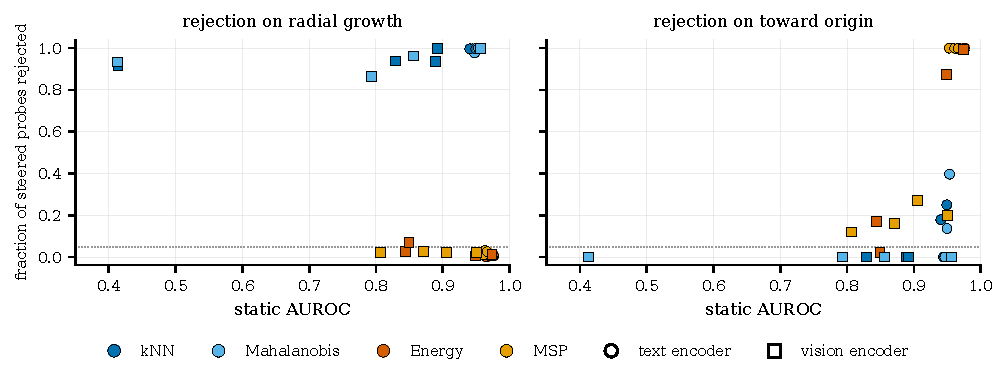
\includegraphics[width=\linewidth]{figures/fig_teaser.pdf}
\caption{Static AUROC against rejection of steered ID probes at the matched horizon, one point per detector and encoder (mean over three seeds). The detectors with the best static AUROC are the logit-based scores, which almost never reject radially grown probes; distance-based scores reject nearly all of them, even where their static AUROC is below chance. The dotted line marks the target rate $\tau$.}
\label{fig:teaser}
\end{figure}
Table~\ref{tab:static} shows that a logit-based score has the highest static AUROC for every encoder: energy
for all but one, and MSP for the remaining one. On radial growth, however, logit-based scores almost never
reject steered probes, while distance-based scores reject nearly all of them (Figure~\ref{fig:teaser}). The
ranking also inverts in the other direction. On ResNet-18, kNN is below chance statically, driven by SVHN,
yet it rejects the large majority of radially grown probes.

A single benchmark number therefore does not determine which shifts a detector misses. This is consistent
with the argument that supervised detectors answer proxy questions~\citep{li2025wrong}. Steering
localises those proxies along declared paths.

\begin{table}[t]
\centering
\small
\caption{Static OOD detection (AUROC, mean $\pm$ SD over three seeds); best per encoder in bold.
Vision AUROC pools CIFAR-100 and SVHN.}
\label{tab:static}
\begin{tabular}{lcccc}
\toprule
encoder & kNN & Mahalanobis & Energy & MSP \\
\midrule
MPNet & 0.948$\pm$0.001 & 0.948$\pm$0.001 & \textbf{0.976$\pm$0.000} & 0.963$\pm$0.001 \\
MiniLM-L6 & 0.944$\pm$0.001 & 0.946$\pm$0.000 & \textbf{0.965$\pm$0.000} & 0.953$\pm$0.001 \\
BGE-base & 0.940$\pm$0.001 & 0.950$\pm$0.001 & \textbf{0.971$\pm$0.001} & 0.961$\pm$0.001 \\
BGE-large & 0.949$\pm$0.001 & 0.953$\pm$0.001 & \textbf{0.976$\pm$0.001} & 0.966$\pm$0.001 \\
\midrule
ResNet-18 & 0.414$\pm$0.007 & 0.413$\pm$0.000 & \textbf{0.844$\pm$0.014} & 0.806$\pm$0.009 \\
ResNet-50 & 0.829$\pm$0.001 & 0.794$\pm$0.004 & 0.849$\pm$0.005 & \textbf{0.871$\pm$0.002} \\
ViT-B/16 & 0.889$\pm$0.002 & 0.856$\pm$0.005 & \textbf{0.949$\pm$0.003} & 0.905$\pm$0.009 \\
DINOv2-S & 0.892$\pm$0.002 & 0.957$\pm$0.002 & \textbf{0.974$\pm$0.003} & 0.950$\pm$0.004 \\
\bottomrule
\end{tabular}
\end{table}





\subsection{RQ2: Do distance- and logit-based detectors fail along different paths?}
\begin{figure}[t]
\centering
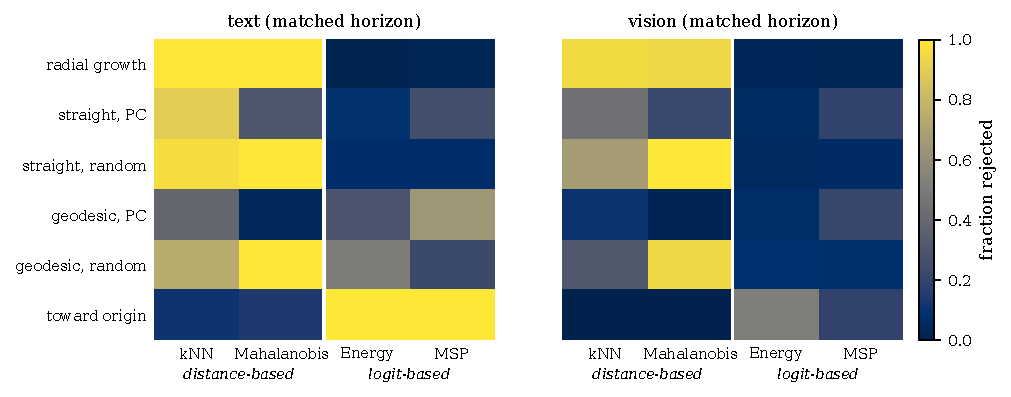
\includegraphics[width=\linewidth]{figures/fig_failure_map.pdf}
\caption{Rejection of steered ID probes at the matched horizon for every path family and detector, averaged over three seeds and four encoders per modality. Distance-based scores fail toward the origin; logit-based scores fail under radial growth and straight rays.}
\label{fig:failuremap}
\end{figure}
They do, and the pattern follows the norm (Figure~\ref{fig:failuremap}; numeric values with confidence
intervals in Table~\ref{tab:matched} and rejection curves in Figure~\ref{fig:curvesseeds}).
\begin{itemize}
\item \emph{Radial growth: distance-based scores reject more than logit-based scores.} Each comparison
(kNN and Mahalanobis vs.\ energy, kNN vs.\ MSP) is significant in every (seed, encoder) cell in both
modalities, and the differences are close to the largest possible.
\item \emph{Toward the origin: logit-based scores reject more than distance-based scores.} In text the
difference is large and significant in every cell. In vision, energy's advantage is significant in most
cells, and no cell shows a difference in the opposite direction. The only non-significant cells are
ResNet-50 in each seed, whose origin Proposition~\ref{prop:radial} predicts to be accepted by energy.
\item \emph{Straight rays.} These both grow the norm and rotate the direction, and behave like radial
growth: energy rarely rejects them, while kNN rejects a large share of them.
\end{itemize}
The vision energy result is bimodal across encoders (Table~\ref{tab:perencoder}): rejection toward the origin
is high for ViT-B/16, near-complete for DINOv2-S and rare for the two ResNets. Both low cases are explained.
ResNet-50's origin is predicted to be accepted, and ResNet-18's paths stop far from the origin because of
the horizon cap.

\subsection{RQ3: Does Proposition~\ref{prop:radial} predict the decisions?}
\begin{figure}[t]
\centering
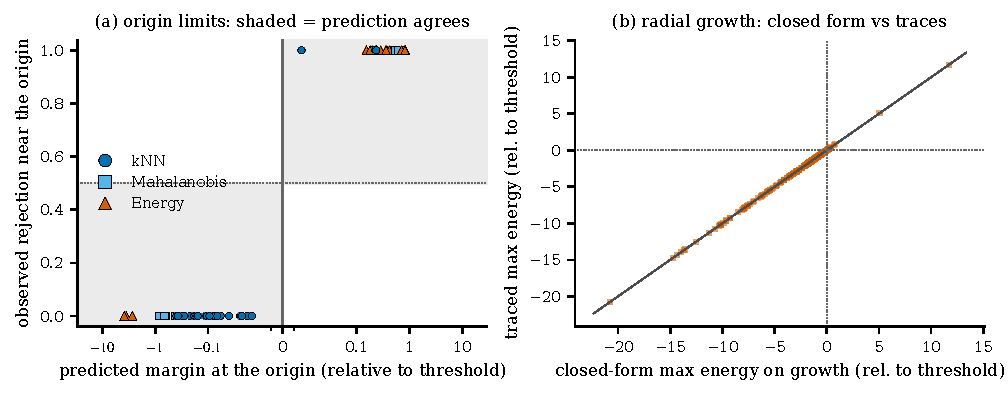
\includegraphics[width=\linewidth]{figures/fig_theory.pdf}
\caption{(a) Predicted margin of each detector's decision at the origin (Proposition~\ref{prop:radial}) against the observed rejection of probes that reach it, for every seed, encoder and (for kNN) decisive reference fit; shaded quadrants mark agreement. (b) Closed-form maximum energy along radial growth against the maximum traced on the grid, per probe (first seed); the line is the identity.}
\label{fig:theory}
\end{figure}
All origin conditions (a)--(d) match the observed decisions in every (seed, encoder) cell:
\begin{itemize}
\item \emph{Energy}, including ResNet-50, whose threshold exceeds $-\lse(b)$, so its origin is accepted.
\item \emph{kNN.} The general condition $c_k\le c^*$ holds on every reference fit. We test only
(fit, probe) pairs whose margin $|r_{(k)}-t|$ exceeds the endpoint norm, where the 1-Lipschitz bound makes
the observation decisive; thousands of pairs qualify. The unit-norm special case $c_k<1/2$ fails for
ResNet-18 and ResNet-50, whose neighbours are strongly aligned but whose smallest reference norms are small.
\item \emph{Radial growth.} The closed-form energy condition of (a) matches the traces for every probe,
and growth causes no new energy rejection.
\end{itemize}
Figure~\ref{fig:theory} shows both checks: every observation falls in the quadrant its predicted margin
assigns, and the closed-form maximum energy along radial growth coincides with the traced maximum. The two
cases a naive reading would call exceptions are both predicted. The anisotropic BGE encoders reject
the origin under both distance scores, and ResNet-50's energy accepts it.

\subsection{RQ4: What happens when the norm is held fixed?}
\begin{figure}[t]
\centering
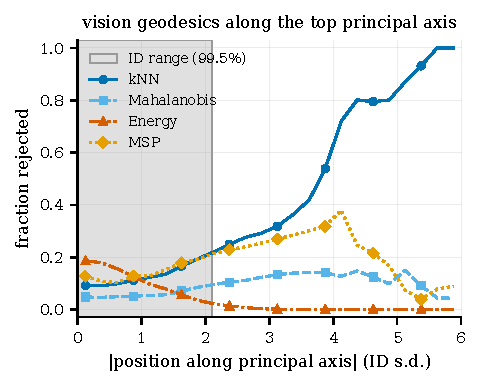
\includegraphics[width=.62\linewidth]{figures/fig_support.pdf}
\caption{Vision geodesics along the top principal axis (first seed): rejection as a function of the distance travelled along the axis, in ID standard deviations measured on the ID test split. The shaded band is the ID range. Energy stops rejecting as the paths leave it, while kNN rises.}
\label{fig:support}
\end{figure}
On geodesics no family is uniformly blind. Mahalanobis rejects nearly all random geodesics, whereas energy
rejects few of them in vision and about half in text. In vision, principal-axis geodesics are rarely rejected
by any detector at the matched horizon; in text, MSP rejects most of them and kNN a substantial share. We
test whether the vision paths leave the ID data at all.

An independent check on the first seed uses only the ID test split, which no detector uses. At the matched
horizon, vision endpoints lie just beyond the edge of the ID range along the steering axis and well within
the Mahalanobis acceptance region. These paths are therefore close to ID-preserving at $\alpha_m$. Once they
move clearly outside the ID range along the axis (Figure~\ref{fig:support}), energy flags none of these points, MSP and Mahalanobis flag
a minority, and kNN catches a substantial share. This is a failure shared by the logit scores and largely by
Mahalanobis; the kNN score catches part of it.

\subsection{RQ5: Do natural input transformations realise these paths?}
\begin{figure}[t]
\centering
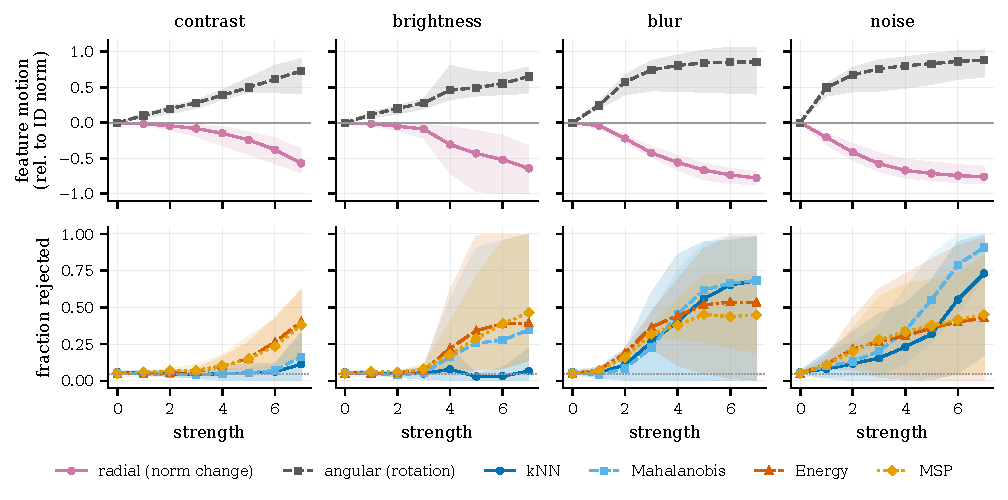
\includegraphics[width=\linewidth]{figures/fig_realise.pdf}
\caption{Feature motion and detector response under natural transformations of CIFAR-10 test images (vision encoders, first seed; lines are encoder means, bands the range across encoders). Top: radial and angular components of the feature displacement, relative to the ID norm. Bottom: rejection at the calibrated thresholds. Every transformation shrinks the norm and rotates the features.}
\label{fig:realise}
\end{figure}
Lemma~\ref{lem:reduction} transfers blindness from a feature path to every input shift that realises
it, so we ask which feature motions real shifts produce. We apply four natural transformations of
increasing strength to ID test images (contrast reduction, darkening, blur and additive noise), encode
them, and split each feature displacement into a radial and an angular component
(Figure~\ref{fig:realise}).
\begin{itemize}
\item Every transformation \emph{shrinks} the feature norm while rotating the features. Real shifts
therefore occupy the shrink-and-rotate cell of Table~\ref{tab:polar}, which our designed paths reach only
transiently.
\item Under contrast and brightness changes, shrinkage dominates at moderate strength. There the
logit-based scores respond first, while kNN stays close to the target rate, as
Proposition~\ref{prop:radial} predicts for shrinking norms.
\item Under blur and noise, rotation is much larger. Every detector responds, and the distance-based
scores overtake the logit-based ones at the highest strengths.
\end{itemize}
These transformations are covariate shifts of ID images rather than semantic OOD. They show that the
radial and angular motions we steer along are produced by ordinary input changes, and that the predicted
complementarity appears there too.

\subsection{RQ6: Is the energy decision a property of the predictor?}
\begin{figure}[t]
\centering
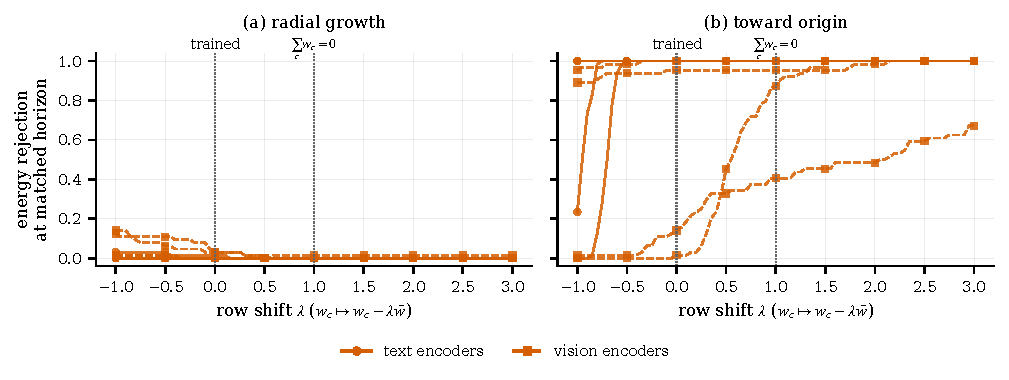
\includegraphics[width=\linewidth]{figures/fig_gauge.pdf}
\caption{Energy rejection at the matched horizon as every row of the trained head is shifted by a multiple $\lambda$ of the mean row (first seed). All predictions are unchanged for every $\lambda$ (checked on the ID test set). Toward the origin, the decision changes substantially with $\lambda$; under radial growth, energy rejection stays low throughout.}
\label{fig:gauge}
\end{figure}
Proposition~\ref{prop:gauge} says that energy depends on a component of the head that no prediction
reveals. We sweep this component on the trained heads by replacing $w_c$ with $w_c-\lambda\bar w$, where
$\bar w$ is the mean row, and recalibrate energy at each $\lambda$ (Figure~\ref{fig:gauge}). Toward the
origin, energy's rejection changes substantially with $\lambda$ for several encoders, in both modalities,
although every prediction is identical. Under radial growth it stays low throughout. A head
with the same predictions can therefore yield a different energy detector, while its blindness to norm
growth persists.

\subsection{Real distribution shifts}
\hole{Norm link: currently a single case.} Relative to ID features (first seed):
\begin{itemize}
\item CLINC out-of-scope queries have exactly the ID norm, because the encoders normalise.
\item CIFAR-100 features have nearly the ID norm.
\item SVHN features are clearly smaller for ResNet-18, slightly smaller for DINOv2-S, and slightly larger
for ResNet-50 and ViT-B/16.
\end{itemize}
The one strongly norm-shrinking case, ResNet-18 on SVHN, shows the complementarity predicted by
Proposition~\ref{prop:radial}: energy detects SVHN well, while kNN is below chance. Across all
(encoder, OOD set) pairs, the norm ratio does not predict the energy-over-distance gap
(Figure~\ref{fig:realood}).

\section{Limitations}
\begin{itemize}
\item The analysis covers linear heads on frozen encoders, at a single calibration level.
\item Feature-space paths are not claimed to be realised by input-space shifts. Lemma~\ref{lem:reduction}
transfers blindness only to shifts that do realise them.
\item The shrink-and-rotate cell of Table~\ref{tab:polar} is reached by natural transformations
(RQ5) but not yet by a designed path family, and RQ5 covers vision only.
\item The horizon is a development choice, and paths toward the origin cannot reach it for all probes.
\item Energy decisions depend on a prediction-invariant component of the head
(Proposition~\ref{prop:gauge}); our energy results are specific to the trained heads, and RQ6 shows how
much they move under one family of row shifts.
\item The link to real shifts rests on one encoder--dataset pair.
\end{itemize}

\appendix
\section{Implementation details}\label{app:impl}
\begin{table}[!htbp]
\centering
\small
\caption{Settings used for every reported result.}
\label{tab:impl}
\begin{tabular}{ll}
\toprule
setting & value \\
\midrule
target ID rejection $\tau$ & 0.05 (order statistic $\lceil(m+1)(1-\tau)\rceil$) \\
kNN neighbours $k$ & 5 (Euclidean, unnormalised) \\
energy / MSP temperature & 1 \\
horizon $H$ & $3\bar r$ (median ID radius of $\mathcal{D}$) \\
toward-origin stop & $0.99\min_{z\in\mathcal{P}}\|z\|$ \\
geodesic cap & arc length $0.95\pi\min_{z\in\mathcal{P}}\|z\|$ \\
grid / bisection & 101 points / 15 steps \\
resamples of $\mathcal{D}$ / $\mathcal{V}$ & 6 / 6 (radial families: 1 direction, 1 sign) \\
probes per encoder and seed & 64 \\
seeds & 3 (split, head and draws vary together) \\
matched horizon $\alpha_m$ & $1.04\,\bar r$ (text), $0.75\,\bar r$ (vision) \\
confidence intervals / tests & 95\% hierarchical bootstrap / one-sided paired bootstrap, $p<0.05$ \\
linear head & AdamW, learning rate 0.01, weight decay $10^{-4}$, 30 epochs, batch 128 \\
CLINC150 pools per intent & 60 / 20 / 20 train (head / ref.\ / dir.), 10 / 10 val.\ (cal.\ / probes) \\
CLINC150 test (seed 0) & 4498 ID, 1000 out-of-scope (after deduplication) \\
CIFAR-10 pools per class & 500 / 100 / 100 / 100 / 20 (head / ref.\ / dir.\ / cal.\ / probes) \\
vision test (seed 0) & 5000 CIFAR-10, 5000 CIFAR-100, 5000 SVHN \\
feature dimensions & MPNet 768, MiniLM 384, BGE-base 768, BGE-large 1024, \\
 & ResNet-18 512, ResNet-50 2048, ViT-B/16 768, DINOv2-S 384 \\
verification tolerances & recompute $\le1.5\times10^{-11}$; norm drift on geodesics $\le10^{-7}$ \\
compute & $\approx$410 CPU core-hours for the grid; encoding on one GPU \\
\bottomrule
\end{tabular}
\end{table}

\section{Additional results}
\begin{table}[!htbp]
\centering
\small
\caption{Rejection at the matched horizon $\alpha_m$, averaged over three seeds and four encoders per modality,
with hierarchical bootstrap confidence intervals (encoders, then seeds within encoder). Seeds vary the data
split, head training and bootstrap draws together; seed-to-seed variation is small in every cell.
Per-encoder values for the radial paths are in Table~\ref{tab:perencoder}.}
\label{tab:matched}
\begin{tabular}{lcccc}
\toprule
\multicolumn{5}{l}{\emph{text}}\\
path & kNN & Maha & Energy & MSP \\
\midrule
radial growth & 1.00 \,[0.99,\,1.00] & 0.99 \,[0.98,\,1.00] & 0.01 \,[0.00,\,0.01] & 0.02 \,[0.01,\,0.03] \\
toward origin & 0.11 \,[0.00,\,0.22] & 0.13 \,[0.00,\,0.30] & 1.00 \,[1.00,\,1.00] & 1.00 \,[1.00,\,1.00] \\
straight, PC & 0.89 \,[0.88,\,0.91] & 0.30 \,[0.23,\,0.38] & 0.09 \,[0.07,\,0.12] & 0.25 \,[0.22,\,0.28] \\
straight, random & 0.96 \,[0.94,\,0.98] & 1.00 \,[1.00,\,1.00] & 0.07 \,[0.06,\,0.07] & 0.06 \,[0.05,\,0.08] \\
geodesic, PC & 0.39 \,[0.23,\,0.54] & 0.03 \,[0.00,\,0.06] & 0.28 \,[0.15,\,0.46] & 0.64 \,[0.52,\,0.76] \\
geodesic, random & 0.74 \,[0.58,\,0.89] & 1.00 \,[1.00,\,1.00] & 0.51 \,[0.21,\,0.82] & 0.23 \,[0.12,\,0.33] \\
\midrule
\multicolumn{5}{l}{\emph{vision}}\\
path & kNN & Maha & Energy & MSP \\
\midrule
radial growth & 0.95 \,[0.92,\,0.98] & 0.94 \,[0.89,\,0.98] & 0.03 \,[0.01,\,0.06] & 0.02 \,[0.01,\,0.03] \\
toward origin & 0.00 \,[0.00,\,0.00] & 0.00 \,[0.00,\,0.00] & 0.52 \,[0.09,\,0.94] & 0.19 \,[0.13,\,0.25] \\
straight, PC & 0.44 \,[0.28,\,0.68] & 0.22 \,[0.05,\,0.51] & 0.06 \,[0.03,\,0.09] & 0.19 \,[0.11,\,0.27] \\
straight, random & 0.67 \,[0.57,\,0.82] & 1.00 \,[1.00,\,1.00] & 0.05 \,[0.03,\,0.06] & 0.05 \,[0.04,\,0.07] \\
geodesic, PC & 0.10 \,[0.06,\,0.16] & 0.02 \,[0.01,\,0.03] & 0.06 \,[0.03,\,0.09] & 0.21 \,[0.12,\,0.32] \\
geodesic, random & 0.31 \,[0.25,\,0.37] & 0.94 \,[0.85,\,1.00] & 0.08 \,[0.03,\,0.13] & 0.07 \,[0.05,\,0.09] \\
\bottomrule
\end{tabular}
\end{table}
\begin{figure}[!htbp]
\centering
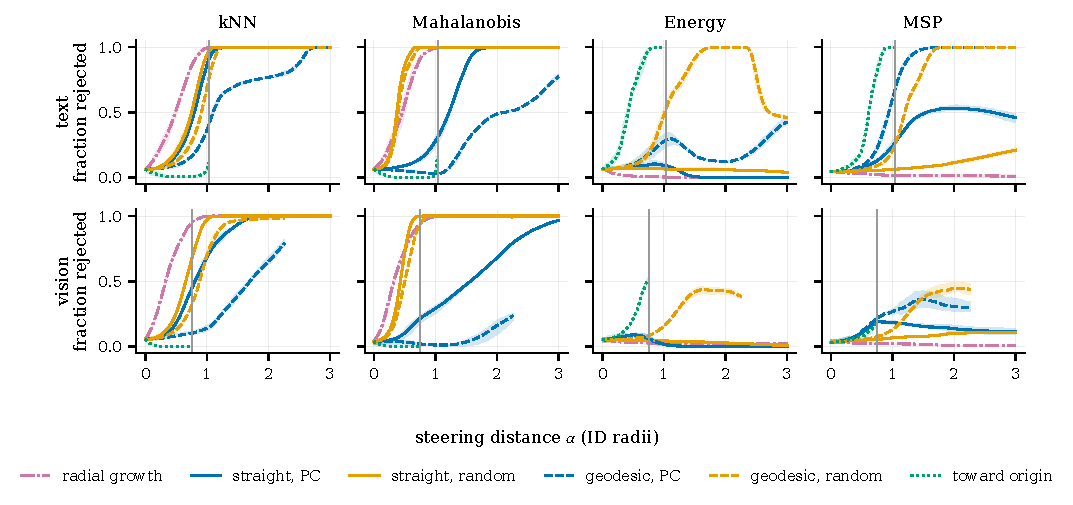
\includegraphics[width=\linewidth]{figures/fig_curves_seeds.pdf}
\caption{Rejection curves $R(\alpha)$ per detector and path family, averaged over encoders; bands show the range across the three seeds. The vertical line marks the matched horizon.}
\label{fig:curvesseeds}
\end{figure}

\begin{figure}[!htbp]
\centering
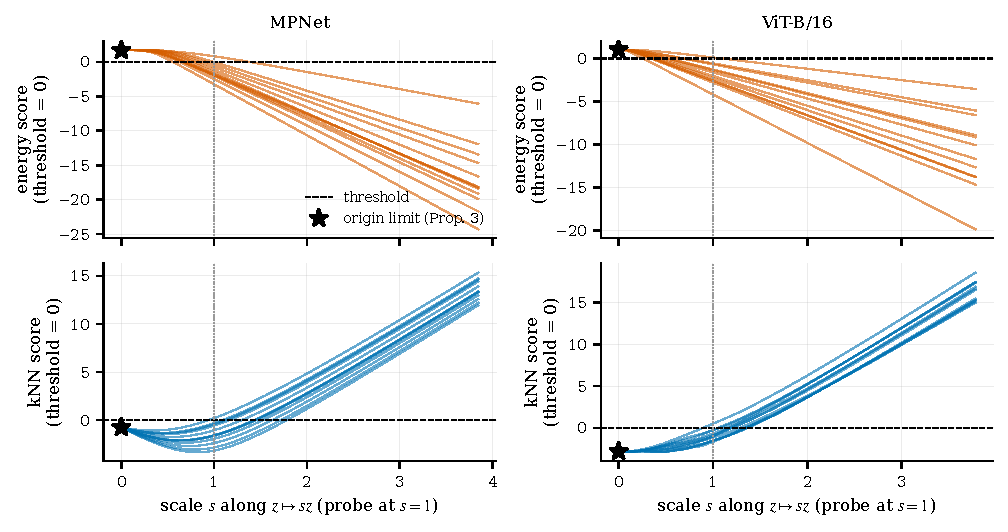
\includegraphics[width=\linewidth]{figures/fig_mechanism.pdf}
\caption{Energy and kNN scores along real radial paths $z\mapsto sz$ for random probes (first seed), shifted so that the calibrated threshold is zero. Stars mark the origin limits of Proposition~\ref{prop:radial}: $-\lse(b)$ for energy and the $k$-th smallest reference norm for kNN.}
\label{fig:mechanism}
\end{figure}

\begin{figure}[!htbp]
\centering
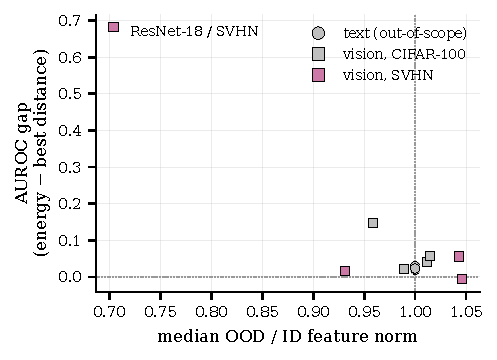
\includegraphics[width=.5\linewidth]{figures/fig_real_ood.pdf}
\caption{Median OOD-to-ID feature norm against the AUROC gap between energy and the best distance score, per encoder and OOD set (first seed).}
\label{fig:realood}
\end{figure}

\section{Per-encoder results}
\begin{table}[!htbp]
\centering
\scriptsize
\caption{Rejection at the matched horizon on the radial paths, per encoder: mean $\pm$ SD over 3 seeds.}
\label{tab:perencoder}
\begin{tabular}{l cccc cccc}
\toprule
 & \multicolumn{4}{c}{radial growth} & \multicolumn{4}{c}{toward origin} \\
encoder & kNN & Maha & Energy & MSP & kNN & Maha & Energy & MSP \\
\midrule
mpnet & 0.99$\pm$0.01 & 0.98$\pm$0.02 & 0.01$\pm$0.01 & 0.03$\pm$0.00 & 0.00$\pm$0.00 & 0.00$\pm$0.00 & 1.00$\pm$0.00 & 1.00$\pm$0.00 \\
minilm & 1.00$\pm$0.01 & 1.00$\pm$0.00 & 0.00$\pm$0.00 & 0.01$\pm$0.01 & 0.00$\pm$0.00 & 0.00$\pm$0.00 & 1.00$\pm$0.00 & 1.00$\pm$0.00 \\
bge\_base & 1.00$\pm$0.00 & 1.00$\pm$0.00 & 0.01$\pm$0.01 & 0.01$\pm$0.01 & 0.18$\pm$0.02 & 0.14$\pm$0.11 & 1.00$\pm$0.00 & 1.00$\pm$0.00 \\
bge\_large & 1.00$\pm$0.00 & 1.00$\pm$0.00 & 0.01$\pm$0.01 & 0.03$\pm$0.01 & 0.25$\pm$0.03 & 0.40$\pm$0.07 & 1.00$\pm$0.00 & 1.00$\pm$0.00 \\
resnet18 & 0.92$\pm$0.06 & 0.93$\pm$0.03 & 0.03$\pm$0.01 & 0.02$\pm$0.02 & 0.00$\pm$0.00 & 0.00$\pm$0.00 & 0.17$\pm$0.03 & 0.12$\pm$0.02 \\
resnet50 & 0.94$\pm$0.04 & 0.86$\pm$0.03 & 0.07$\pm$0.03 & 0.03$\pm$0.02 & 0.00$\pm$0.00 & 0.00$\pm$0.00 & 0.02$\pm$0.01 & 0.16$\pm$0.05 \\
vit\_b16 & 0.93$\pm$0.00 & 0.96$\pm$0.01 & 0.01$\pm$0.01 & 0.02$\pm$0.02 & 0.00$\pm$0.00 & 0.00$\pm$0.00 & 0.88$\pm$0.08 & 0.27$\pm$0.04 \\
dinov2\_s & 1.00$\pm$0.00 & 1.00$\pm$0.00 & 0.01$\pm$0.02 & 0.02$\pm$0.02 & 0.00$\pm$0.00 & 0.00$\pm$0.00 & 0.99$\pm$0.01 & 0.20$\pm$0.05 \\
\bottomrule
\end{tabular}
\end{table}

\section{Proofs}
\hole{Lemma~\ref{lem:reduction}; Prop.~\ref{prop:radial} (a)--(d); Thm.~\ref{thm:cone}; see THEORY.md.}

\bibliographystyle{plainnat}
\bibliography{references}

\end{document}
